\documentclass{article}
% --- watermark (auto-inserted) ---
\usepackage{xcolor}
\usepackage{xfp}% \fpeval; in the kernel since 2022, harmless on older LaTeX
\usepackage{draftwatermark}
\newlength{\watermarkTextWidth}
\AddToHook{begindocument/end}{%
  \SetWatermarkText{\normalfont Generated by The Agentic Scientist}%
  \SetWatermarkFontSize{10pt}%
  \SetWatermarkLightness{0.85}%
  \settowidth{\watermarkTextWidth}{\normalfont\fontsize{10pt}{12pt}\selectfont Generated by The Agentic Scientist}%
  \edef\watermarkScale{\fpeval{0.8 * sqrt(\paperwidth**2 + \paperheight**2) / \watermarkTextWidth}}%
  \edef\watermarkAngle{\fpeval{atand(\paperheight/\paperwidth)}}%
  \SetWatermarkScale{\watermarkScale}%
  \SetWatermarkAngle{\watermarkAngle}%
}
% --- end watermark ---

\usepackage{iclr2026_conference,times}
\usepackage[T1]{fontenc}
\usepackage[utf8]{inputenc}
\usepackage{amsmath,amssymb,booktabs,graphicx,url,hyperref}
\usepackage{subcaption}
\title{Score-Targeted Subsets for Predicting LLM Benchmark Accuracy}
\author{}
\newcommand{\clip}{\operatorname{clip}_{[0,1]}}
\newcommand{\sigmoid}{\operatorname{sigmoid}}

\begin{document}
\maketitle

\begin{abstract}
Historical item-level evaluations offer a way to estimate a language model's benchmark accuracy without evaluating every item. We examine a frozen subset-and-decoder package that targets covariance with full-benchmark accuracy, rather than item representativeness alone. Its source-trained, nested query path is shared across target models; a source-selected decoder maps observed responses to estimated full scores. Recorded held-out evaluations cover nine benchmark matrices, three seeds, and budgets of 5, 10, and 25 items. The package attains mean absolute error of 3.90 percentage points, compared with 5.91 for a local item-response estimator and 10.52 for uniform sampling. A paired lineage-block interval for its error difference from local item response is $[-2.57,-1.46]$ percentage points, conditional on these benchmarks. However, the comparison reverses on several benchmark--budget combinations, including every evaluated budget on HELM MATH. These results support an average package-level advantage within the frozen snapshot, not universal superiority, isolated component effects, or guaranteed transfer to new model families.
% @evidence[[paper_data.json#/final_evaluation/metrics]]
% @evidence[[analysis/paper_statistics.json#/uncertainty]]
% @evidence[[analysis/paper_statistics.json#/local_irt_reversals]]
\end{abstract}

\section{Introduction}
Evaluating a language model throughout training or across prompting configurations repeatedly measures an entire benchmark, even when only its aggregate accuracy is needed. Historical evaluations contain more information than a list of aggregate scores: each item supplies a response pattern across source models. Such patterns can identify items whose outcomes are informative about an unseen model's full score. The practical question is not merely whether a benchmark can be compressed, but what should be preserved by the compression and how failures should be detected.

An item subset that represents typical response patterns need not be the subset that best predicts the mean. Some diverse items may contribute little information about differences in full accuracy; conversely, strongly correlated items can be redundant once another item has been observed. This motivates a score-directed criterion: select an item by its remaining covariance with the full score, relative to its conditional variance. A decoder can then use the complete observed response vector, rather than interpreting the queried fraction as an ordinary miniature test.

We study this principle through a frozen acquisition-and-decoding package and paired local comparators. The source-trained query path is common to all target models, while the predicted score depends on each target's answers. This is nonadaptive item selection with respect to target responses. It is not a target-specific testing policy, and it does not require item text or target-model identity at inference. The readable implementation also contains a source-selected nonlinear decoding option, but the retained evaluation does not establish which decoder branch was active for each case. Our scientific object is therefore the complete evaluated package, not a claimed nonlinear mechanism.

The contributions are deliberately bounded. We describe the score-directed acquisition objective and compatible score decoding in the supplied source counterpart. We reconcile the recorded held-out predictions with aggregate accuracy and lineage-level ranking metrics, using budget-matched local baselines. Finally, we show where the aggregate advantage breaks down and distinguish fixed-benchmark uncertainty from evidence about unseen benchmarks. No controlled component ablations are available, so no part of the comparison identifies the isolated benefit of acquisition, linear decoding, or nonlinear residual correction.

Across the retained evaluation, lower average error coexists with unfavorable comparisons on HELM MATH, LegalBench, and MedQA at particular budgets. Those reversals are central evidence, not exceptions to be removed. A useful compact evaluator must be assessed both as an estimator of absolute accuracy and as a ranking device, with its source dependence and uncertainty made explicit.
% @evidence[[analysis/paper_statistics.json#/local_irt_reversals]]

\begin{figure}[t]
\centering
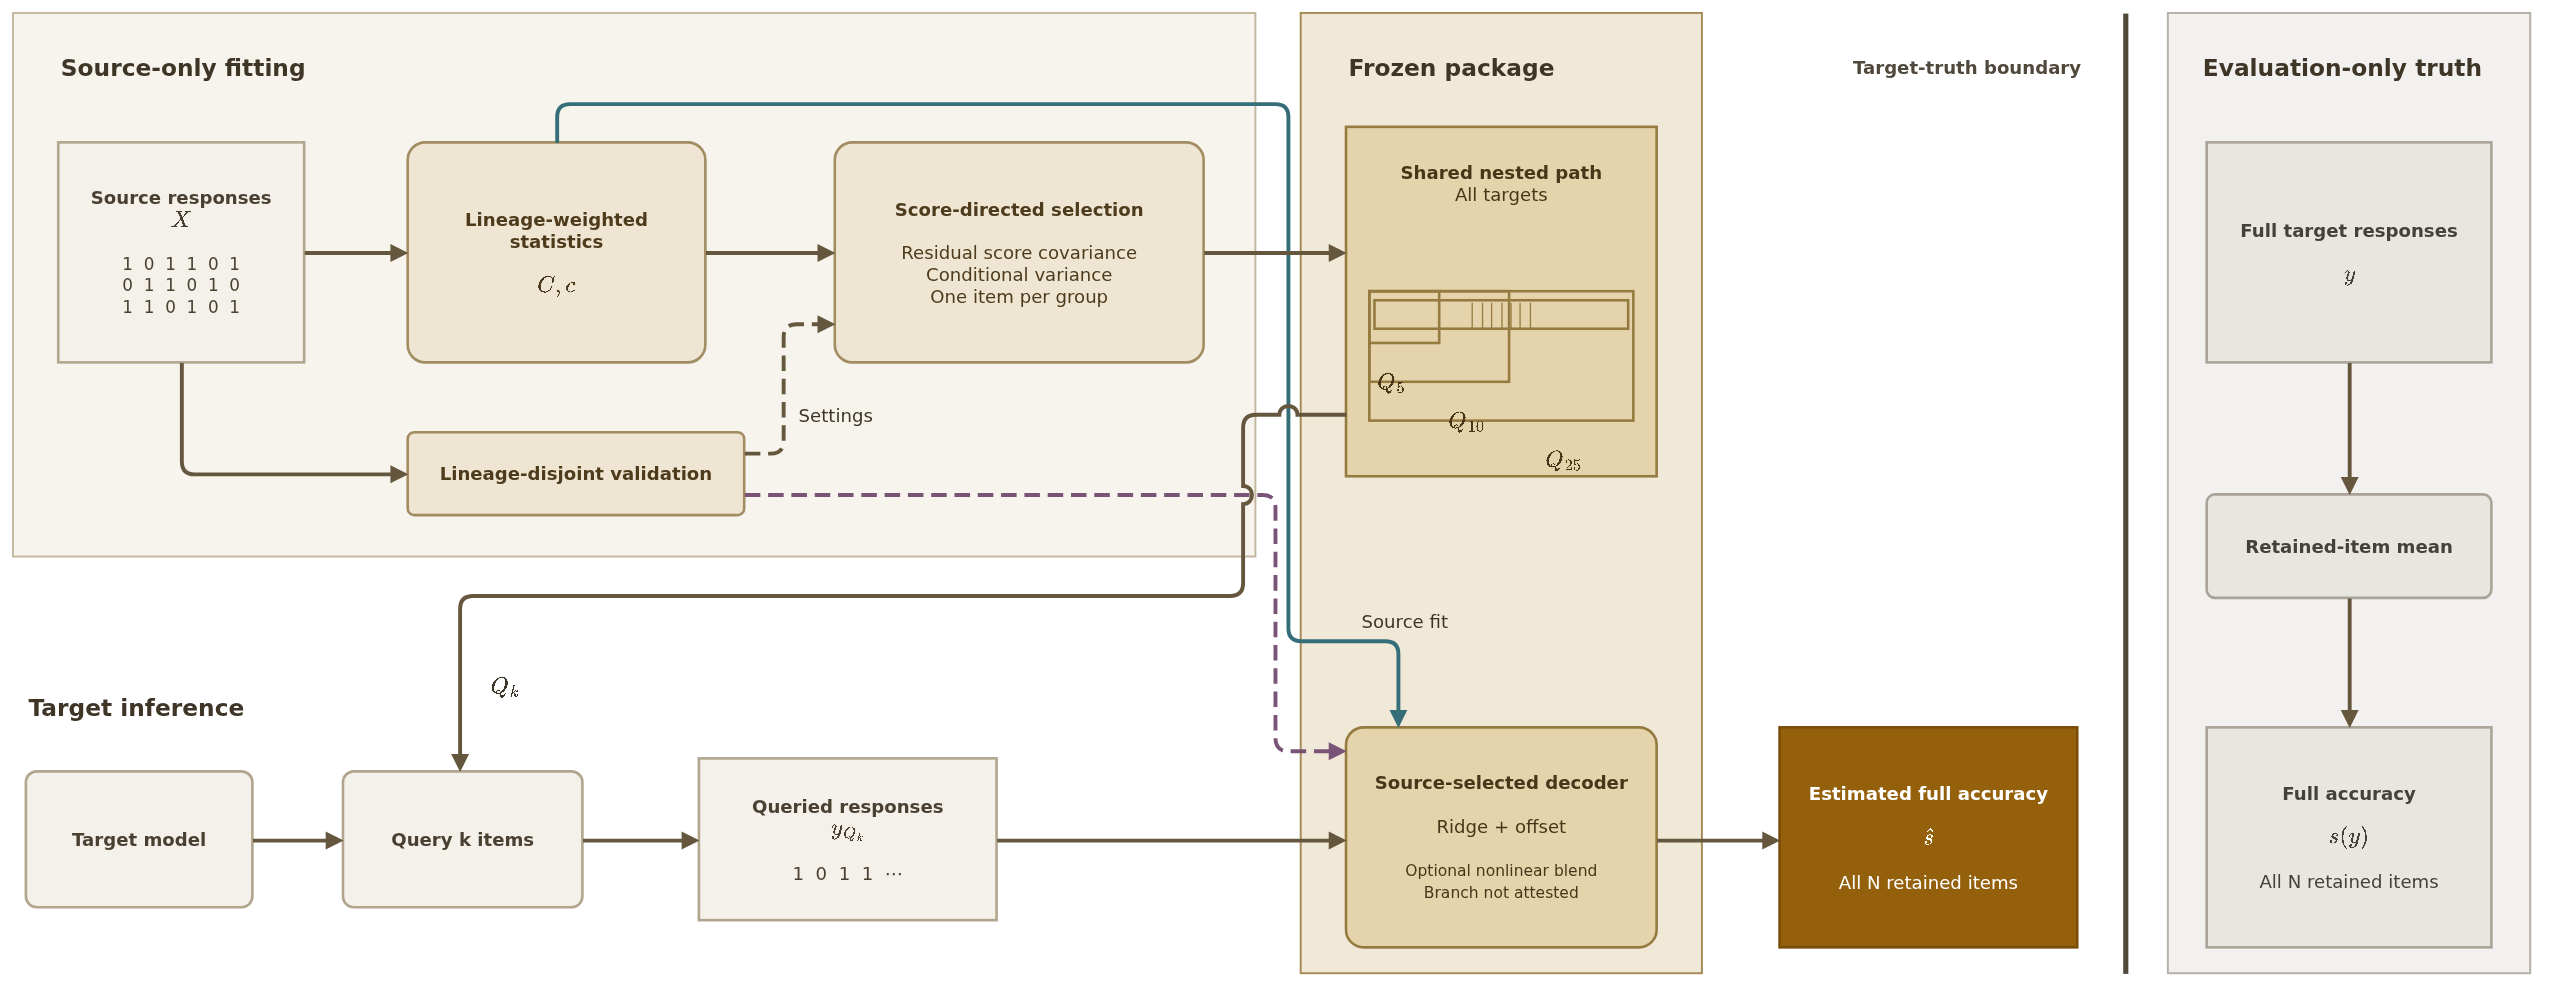
\includegraphics[width=\textwidth,height=2in,keepaspectratio]{figures/score_prediction_overview.png}
\caption{Estimation setting and information boundary. Source response matrices determine a shared score-directed item path and source-selected decoder. Only the target responses at the queried items enter prediction; retained full-benchmark target scores are used for evaluation. The optional decoder branch is not independently attested per case.}
\label{fig:overview}
\end{figure}

\section{Related Work}
\paragraph{Compact benchmark evaluation.}
Anchor Points uses correlations in model responses to construct small representative evaluation sets \citep{Vivek2024}. tinyBenchmarks studies curated subsets and score estimation across established evaluation suites \citep{Polo2024}; metabench compresses reasoning and knowledge tests using informative items and ability estimates \citep{Kipnis2025}. These works motivate source-response reuse, but their reported results are not experimental baselines here. Our anchor and item-response comparators are the specific local implementations described below, not reproductions of every feature of those systems.

Supervised assessors can predict a new model's performance from its responses on reference instances and features of the instance to be predicted \citep{Pacchiardi2024}. Our setting instead predicts the aggregate score directly from binary response histories, without using item-text features. Learned acquisition policies offer another route to efficient evaluation \citep{Li2025}. In contrast, the item path considered here is fixed from source data before target responses arrive. Adaptive evaluation with continuous bounded scores \citep{Balkir2026} addresses a broader observation model and stopping problem; our evidence is restricted to fixed-budget binary matrices. ONEBench studies aggregation over heterogeneous, incomplete evaluations \citep{Ghosh2024}, whereas the present target is a retained benchmark's arithmetic mean.

\paragraph{Targeted design and regularization.}
Selecting measurements for a particular linear functional, rather than estimating all parameters equally well, is a classical experimental-design distinction \citep{Elfving1952}. The score-directed criterion below is an empirical, regularized covariance construction, not a claim to solve that general design problem optimally. Ridge regularization stabilizes regression when observations are correlated \citep{Hoerl1970}. Here both the acquisition criterion and decoder depend on source-derived covariance, making source-to-target stability an empirical assumption rather than a consequence of regularization.

\paragraph{Evaluation discipline.}
Model selection can overfit its own validation criterion \citep{Cawley2010}, and repeated adaptive reuse of evaluation data requires care \citep{Dwork2015}. We consequently separate development feedback from the recorded held-out comparison. Bootstrap uncertainty \citep{Efron1979} is reported under the evaluator's actual resampling unit, not as a distribution-free certificate. None of these methodological connections turns the observed comparison into evidence of universal benchmark predictability.

\section{Method}
\subsection{Problem and Estimation Target}
For one benchmark, let $X\in\{0,1\}^{M\times N}$ contain source-model responses on $N$ retained item columns. A target model has response vector $y\in\{0,1\}^{N}$ and full accuracy
\begin{equation}
s(y)=\frac{1}{N}\sum_{j=1}^{N}y_j.
\label{eq:target}
\end{equation}
Only responses on a subset $Q_k$, of size $k$, are made available to the estimator. The output is $\hat s(y_{Q_k};X)\in[0,1]$. Historical source responses can be used in fitting and tuning; unqueried target responses and full target scores cannot. The target is the mean over retained columns, not a claim to recover an unreconciled original benchmark or a differently weighted official leaderboard score.
% @evidence[[paper_data.json#/final_evaluation/evaluation_evidence/episodes/0/solution/episodes/0/checkpoints]]
% @evidence[[source_evidence/evaluator/evaluate_final.py#L844]]

Source rows have nonnegative weights $w_m$ summing to unity. The supplied protocol gives each metadata-defined source lineage equal total weight and distributes that weight equally among its rows. Item-content groups constrain selection: at most one item from any group is queried. However, all retained columns, including their multiplicities, remain in Equation~\ref{eq:target}. Thus query uniqueness and score weighting are distinct operations. The same nested path $Q_5\subset Q_{10}\subset Q_{25}$ serves all targets within a fitted case.
% @evidence[[source_evidence/evaluator/evaluate_final.py#L556]]
% @evidence[[source_evidence/selected/src/program.py#L99]]

\subsection{Score-Directed Shared Acquisition}
Define the weighted item means $\mu_j=\sum_m w_mX_{mj}$, source full scores $s_m=N^{-1}\sum_jX_{mj}$, and weighted score mean $\bar s=\sum_mw_ms_m$. Let
\begin{equation}
Z_{mj}=\sqrt{w_m}(X_{mj}-\mu_j),\quad
u_m=\sqrt{w_m}(s_m-\bar s),\quad C=Z^\top Z,\quad c=Z^\top u.
\label{eq:covariance}
\end{equation}
The vector $c$ targets full accuracy explicitly. A high item variance alone does not imply a high score covariance; a high marginal covariance can also become redundant after other items are selected.
% @evidence[[source_evidence/selected/src/surrogate.py#L6]]

For regularization $\lambda>0$, a partial subset $Q$ has regularized score information $c_Q^\top(C_{QQ}+\lambda I)^{-1}c_Q$. A Schur-complement expansion yields the incremental criterion
\begin{equation}
g(j\mid Q)=
\frac{\left[c_j-C_{jQ}(C_{QQ}+\lambda I)^{-1}c_Q\right]^2}
{C_{jj}+\lambda-C_{jQ}(C_{QQ}+\lambda I)^{-1}C_{Qj}}.
\label{eq:gain}
\end{equation}
The readable selector greedily adds the legal item maximizing this quantity, masking every item in an already queried content group. Empty-set terms vanish. This construction optimizes a source empirical linear-prediction surrogate; it neither guarantees target MAE reduction nor proves that the greedy subset is globally optimal. Ridge regularization also changes the acquisition ranking, not merely the final regression fit.
% @evidence[[source_evidence/selected/src/surrogate.py#L31]]

The rationale is to prefer responses that explain residual variation in the quantity actually being estimated. In contrast, response-space coverage can emphasize diversity without accounting for whether that diversity changes the full mean. This is a design hypothesis: the available comparison changes the decoder as well as the query path, so it cannot establish that Equation~\ref{eq:gain} alone explains the measured advantage.

\subsection{All-Observation Score Decoding}
For observed history $z=y_Q$, the linear decoder uses
\begin{align}
\beta_Q&=(C_{QQ}+\lambda I)^{-1}c_Q,\\
\hat s_{\mathrm{ridge}}(z)&=\bar s+(z-\mu_Q)^\top\beta_Q,\qquad
\hat s_{\mathrm{offset}}(z)=\bar s+\frac{1}{|Q|}\sum_{j\in Q}(z_j-\mu_j),\\
\hat s_L(z)&=\clip\left[\alpha\hat s_{\mathrm{ridge}}(z)+(1-\alpha)\hat s_{\mathrm{offset}}(z)\right].
\label{eq:linear}
\end{align}
The offset term corrects the source score mean using the target's average deviation from source item means. Every queried answer contributes to decoding; identical answer histories map to the same prediction. With no observations, the fallback is the source score mean. Clipping bounds predictions but does not supply confidence intervals or unbiasedness.
% @evidence[[source_evidence/selected/src/surrogate.py#L75]]

The supplied implementation also admits an optional decoder that infers a regularized scalar log-odds shift from queried answers, averages its predicted probabilities over retained items, and adds a source-fitted residual ridge correction. It can blend this estimate with Equation~\ref{eq:linear}, including a purely linear fallback. Its residual features and fitted shifts use the same query prefix during training and inference. Supplementary Information gives the equations. Since no per-case branch selections or component ablations are attested, we do not label the measured gain a nonlinear-decoder effect.
% @evidence[[source_evidence/selected/src/nonlinear_decoder.py#L18]]
% @evidence[[source_evidence/selected/src/nonlinear_decoder.py#L233]]

\subsection{Source-Only Selection of Settings}
Settings are selected with lineage-disjoint source folds. Within each fold, item statistics and the acquisition path are refitted on fitting rows, and accuracy estimates are assessed on held-out source lineages. Loss averages absolute errors over the evaluation prefixes, then gives held-out lineages equal weight. The optional decoder adds an outer source split that refits the linear selector and its tuning within the fitting partition. No target full score is supplied for these choices.
% @evidence[[source_evidence/selected/src/surrogate.py#L111]]
% @evidence[[source_evidence/selected/src/nonlinear_decoder.py#L142]]

The source counterpart is inspectable, but the retained final source-tree digest does not itself prove byte identity with that available tree. We therefore distinguish an implementation-grounded description of the supplied counterpart from the directly attested final predictions. This boundary is particularly important for settings or conditional branches absent from the measurement records. The empirical conclusions below require the recorded predictions, not an assumption about which optional branch produced them.
% @evidence[[source_evidence/inventory.json]]
% @evidence[[paper_data.json#/final_evaluation/program_tree_sha256]]

\section{Experimental Protocol}
\subsection{Data, Splits, and Budget Matching}
The recorded final evaluation covers nine binary benchmark matrices. The leaderboard-derived group contains BBH \citep{Suzgun2022}, GPQA \citep{Rein2023}, MMLU-Pro \citep{Wang2024}, MuSR \citep{Sprague2023}, and a MATH subset \citep{Hendrycks2021}. The HELM-derived group \citep{Liang2023} contains LegalBench \citep{Guha2023}, MATH, MedQA \citep{Jin2020}, and MMLU \citep{Hendrycks2020}. These are the supplied retained matrices, not newly collected LLM outputs. Distinguishing leaderboard MATH from HELM MATH is essential because they are separate evaluation cases.
% @evidence[[paper_data.json#/final_evaluation/evaluation_evidence/episodes]]

Development feedback concerned ARC-Challenge, IFEval, Commonsense, and GSM matrices; it is not pooled with the final metrics. The frozen package is refitted from the source rows of each final benchmark. Hence this is evaluation across held-out benchmark cases with per-benchmark source fitting, not transfer of a single fixed set of coefficients across tasks. No additional evaluated task family is supplied beyond this benchmark-prediction setting.
% @evidence[[paper_data.json#/best_correct/evaluation_evidence/episodes]]

The frozen resource manifests describe model-lineage separation and conservative item-content reconciliation across development and final data. Anonymous group identifiers, rather than model names or item text, reach the estimator. Known aliases and declared base-model relations guide grouping; undocumented derivatives can remain related across partitions. Common-stem normalization likewise does not establish semantic or pretraining disjointness. These are metadata-based safeguards, not proof of independent source and target populations.
% @evidence[[source_evidence/manifests/bbh_manifest.json#/lineage_policy]]
% @evidence[[source_evidence/manifests/bbh_manifest.json#/limitations]]

Evaluation uses seeds 1009, 2003, and 3001 and cumulative query budgets 5, 10, and 25. This yields 81 non-replay benchmark--budget--seed cells. Each reset discards fitted state. A repeated normal BBH record checks deterministic replay but is excluded from performance averages. Identical-history and duplicated-target checks assess prediction consistency; additional perturbed observations are reported separately, not counted as ordinary performance measurements.
% @evidence[[analysis/paper_statistics.json#/cell_count]]
% @evidence[[paper_data.json#/final_evaluation/evaluation_evidence/episodes]]

\subsection{Compared Estimators}
All nonzero-cost estimators use the same reported item budget, but not necessarily the same items or fitting cost. The \textbf{source prior} returns the weighted source mean and uses no target answers. \textbf{Uniform sampling} selects a random prefix of content-group representatives and scales observed outcomes by each group's retained-column mass. Its clipped, group-mass-weighted estimate is not simply an unweighted mean when group sizes differ. \textbf{Local anchors} constructs normalized source response embeddings, chooses representatives by a farthest-point rule, assigns all retained items to selected representatives, and uses assignment masses to weight their target outcomes. This is a local anchor estimator rather than an exact published Anchor Points reproduction.
% @evidence[[source_evidence/evaluator/evaluate_final.py#L580]]
% @evidence[[source_evidence/evaluator/evaluate_final.py#L598]]

\textbf{Local IRT} uses a logistic ability--difficulty model with regularized ability fitting. It shares the uniform baseline's item path, estimates target ability from the queried answers, and averages predicted probabilities across retained items. Its source-fitted difficulties and implementation details are specified in Supplementary Information. The \textbf{score-targeted package} changes both selection and decoding. Accordingly its comparison with IRT is a package comparison at matched observation budgets, not a selector-only or decoder-only ablation. None of the local comparators establishes a state-of-the-art comparison with the full published systems.
% @evidence[[source_evidence/evaluator/evaluate_final.py#L636]]

\subsection{Metrics and Conditional Uncertainty}
Within each cell, each target lineage receives equal total weight, distributed equally among its models. MAE is the resulting weighted absolute error, and RMSE is the square root of weighted squared error. Ranking metrics are Spearman correlation and Kendall's $\tau_b$ between lineage-mean predictions and lineage-mean true scores, not correlations over individual rows. Aggregate metrics average cells equally, giving each benchmark, budget, and seed equal weight. In particular, aggregate RMSE is a mean of cell RMSEs, not a pooled squared-error statistic.
% @evidence[[source_evidence/evaluator/evaluate_final.py#L556]]
% @evidence[[analysis/paper_statistics.json#/aggregate]]

The evaluator supplies paired percentile intervals from 200 lineage-block bootstrap draws. Within a benchmark, lineage blocks retain their predictions across budgets and seeds; benchmarks retain equal weights. The same aggregate uncertainty object is repeated in the outer seed records and is used only once. These intervals condition on the fixed cases and stored fitting outcomes. They do not resample benchmarks, refit source data, quantify future-family transfer, or provide individual-target prediction intervals. They are the recorded percentile procedure, not higher-order corrected intervals \citep{Efron1987}. No failed normal cells are recorded. The evaluator's completion and qualification outcome are both affirmative; that procedural result does not certify scientific generality.
% @evidence[[analysis/paper_statistics.json#/uncertainty]]
% @evidence[[paper_data.json#/final_evaluation/status]]
% @evidence[[paper_data.json#/final_evaluation/outcome]]

\section{Results}
\subsection{Average Accuracy and Ranking}
Table~\ref{tab:main} reports the frozen final comparison. The score-targeted package has MAE 3.90 percentage points versus 5.91 for local IRT, the strongest recorded aggregate baseline by MAE. Uniform sampling, the source prior, and local anchors have MAE 10.52, 8.34, and 15.67 percentage points, respectively. The package's RMSE is 4.84 percentage points, compared with 7.30 for local IRT. These are averages under the stated weighting, not a guarantee for every target or benchmark.
% @evidence[[paper_data.json#/final_evaluation/metrics]]
% @evidence[[analysis/paper_statistics.json#/aggregate]]

\begin{table}[t]
\centering
\caption{Equal-cell averages over the retained final cases. Error units are percentage points (pp); rank correlations use lineage means. Only the source prior uses no target answers. Baseline RMSE and correlations are reconstructed from the recorded prediction arrays; a constant prior cannot provide a meaningful ranking, so its correlations are omitted.}
\label{tab:main}
% @evidence[[analysis/paper_statistics.json#/aggregate]]
\begin{tabular}{lrrrrr}
\toprule
Estimator & Answers & MAE (pp) & RMSE (pp) & Spearman & Kendall\\
\midrule
Score-targeted package & $k$ & 3.90 & 4.84 & 0.816 & 0.672 \\
Local IRT & $k$ & 5.91 & 7.30 & 0.603 & 0.491 \\
Uniform & $k$ & 10.52 & 12.89 & 0.604 & 0.494 \\
Source prior & 0 & 8.34 & 10.08 & -- & -- \\
Local anchors & $k$ & 15.67 & 18.36 & 0.437 & 0.346 \\
\bottomrule
\end{tabular}

% @evidence[[analysis/paper_statistics.json#/aggregate]]
\end{table}

The mean Spearman correlation is 0.816 for the package, versus 0.603 for local IRT; the corresponding Kendall values are 0.672 and 0.491. Uniform sampling has similar aggregate ranking correlations to local IRT despite substantially higher score error. Thus absolute accuracy estimation and ordering are empirically distinct objectives. Our MAE uncertainty analysis should not be read as a significance test for the differences in either ranking metric. Nor does lineage-level correlation establish that every pair of closely matched individual models is reliably ordered.
% @evidence[[analysis/paper_statistics.json#/aggregate]]

\begin{figure}[t]
\centering
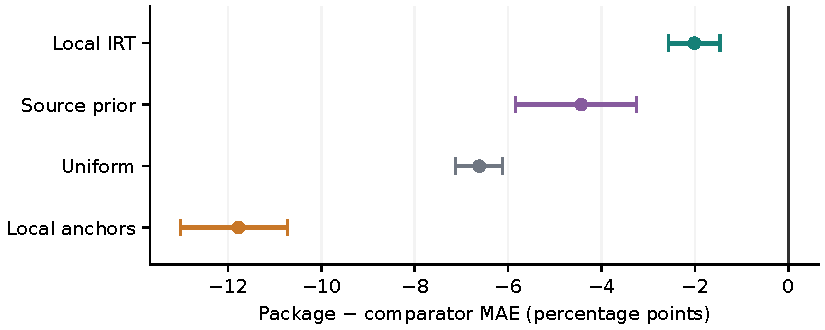
\includegraphics[width=\textwidth]{figures/paired_error_comparison.pdf}
\caption{Paired aggregate MAE differences with the recorded 95\% lineage-block percentile intervals. Negative values favor the score-targeted package. Budgets and seeds remain within each lineage block, and benchmarks are not resampled. All intervals are conditional on the fixed benchmark collection.}
\label{fig:paired}
% @evidence[[analysis/paper_statistics.json#/uncertainty]]
\end{figure}

Figure~\ref{fig:paired} quantifies the aggregate comparisons without discarding their pairing. The package-minus-IRT MAE difference is $-2.01$ percentage points, with interval $[-2.57,-1.46]$. The corresponding differences are $-6.62$ against uniform sampling, $-4.44$ against the prior, and $-11.78$ against local anchors; each recorded interval lies below zero. This is evidence for an average error reduction within the fixed evaluation. It does not estimate the probability that a newly chosen benchmark would favor the package.
% @evidence[[analysis/paper_statistics.json#/uncertainty/comparisons]]

\subsection{Budget Dependence and Seed Consistency}
Averaging over benchmarks and seeds, package MAE decreases from 4.67 percentage points at 5 items to 3.95 at 10 and 3.08 at 25. Local IRT decreases from 7.32 to 5.88 and 4.54, respectively. Package Spearman correlation rises from 0.763 to 0.802 and 0.882 across these budgets. Supplementary Figure~\ref{fig:budget} shows the paired budget profiles alongside the other nonconstant estimators. These are measurements at nested subsets, not a claim of monotonic improvement for each benchmark or every fitted subset.
% @evidence[[analysis/paper_statistics.json#/by_budget]]

The package's aggregate MAEs for the three recorded seeds are 3.816, 4.006, and 3.876 percentage points. Its error is lower than the aggregate local IRT error for each seed. This descriptive consistency is useful, but the seeds reuse the same frozen source and target splits; they are not independent samples of future benchmark environments. Source-prior and deterministic anchor predictions also do not become independent replications merely because their values appear in multiple seed records.
% @evidence[[analysis/paper_statistics.json#/by_seed]]

\subsection{Where the Comparison Reverses}
Figure~\ref{fig:reversals} shows benchmark--budget differences from local IRT, averaging the recorded seeds. On each leaderboard-derived matrix, the package has lower MAE at every evaluated budget. The HELM-derived matrices are mixed: LegalBench favors IRT at 5 and 25 items, HELM MATH favors IRT at all budgets, and MedQA favors IRT at 10 and 25 items. MMLU favors the package across these budgets. These are descriptive cell means; no cell-specific confidence intervals or multiplicity-adjusted tests are supplied.
% @evidence[[analysis/paper_statistics.json#/by_case_budget]]
% @evidence[[analysis/paper_statistics.json#/local_irt_reversals]]

\begin{figure}[t]
\centering
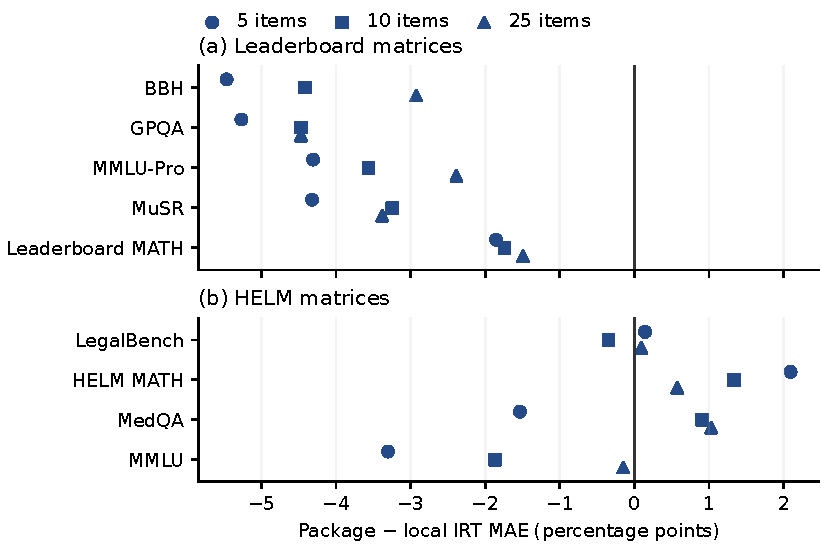
\includegraphics[width=\textwidth]{figures/case_budget_reversals.pdf}
\caption{Benchmark-specific package-minus-local-IRT MAE, averaged over seeds. Shapes distinguish query budgets. Left of zero favors the package; right favors IRT. The shared horizontal scale preserves both the larger leaderboard advantages and the HELM reversals. Panels separate matrix provenance, not independently randomized treatment groups. No benchmark-specific intervals are inferred from the aggregate interval.}
\label{fig:reversals}
% @evidence[[analysis/paper_statistics.json#/by_case_budget]]
\end{figure}

The HELM MATH contrast is substantial enough to matter to the interpretation: at 5 items the package's MAE is 11.63 percentage points, compared with 9.53 for IRT; at 25 items the respective values are 6.19 and 5.61. MedQA is also nonmonotonic for the package: its MAE increases from 6.68 at 5 items to 7.47 at 10, before falling to 5.54 at 25. Additional observations therefore do not ensure lower realized error under a changed regression prefix. We do not diagnose these reversals as saturation, lineage shift, or decoder activation: the retained evidence does not isolate those causes.
% @evidence[[analysis/paper_statistics.json#/by_case_budget/math]]
% @evidence[[analysis/paper_statistics.json#/by_case_budget/med_qa]]

The contrast between matrix groups is likewise not a causal ecosystem effect. Dataset composition, model populations, item reconciliation, and source-target relationships change together. The results support a heterogeneous estimator comparison, not a claim that leaderboard provenance is intrinsically easier to predict. Reporting only the aggregate would conceal meaningful local failures; reporting only the failures would conceal the paired aggregate advantage.

\subsection{Observation Perturbations and Attribution Limits}
When all queried target answers are replaced by zeros, recorded MAE is 21.58 percentage points. Independently rotating each source row's item order while preserving its row mean gives MAE 6.26 percentage points. Both exceed the ordinary-condition 3.90. These interventions are consistent with the package using answer histories and aligned source responses. They do not prove absence of leakage, identify a causal component, or establish that a particular nonlinear module contributes. The all-zero intervention changes observation content rather than measuring real target behavior, and row rotations change the training representation rather than a single decoder component.
% @evidence[[paper_data.json#/final_evaluation/metrics/constant_mae]]
% @evidence[[paper_data.json#/final_evaluation/metrics/permuted_mae]]
% @evidence[[paper_data.json#/final_evaluation/metrics/mae]]
% @evidence[[source_evidence/evaluator/evaluate_final.py#L844]]

No controlled selector/decoder cross-comparison, curve-only decoder result, or residual-only decoder result is available. The most defensible conclusion is therefore that the complete frozen package outperforms the recorded local baselines on average under this protocol. Component attribution remains an unresolved experimental question, even though the readable implementation makes such comparisons possible in future work.

\section{Discussion and Limitations}
\paragraph{Prediction is not benchmark replacement.}
A compact estimate is useful when the target is aggregate accuracy under an already specified evaluation distribution. It cannot recover which unqueried examples failed, measure new capabilities absent from the benchmark, or certify rare-event reliability. HELM explicitly motivates evaluation beyond a single accuracy number \citep{Liang2023}; compressing accuracy must not be presented as compressing all of those desiderata. The present binary-response setting also excludes continuous quality scores and adaptive stopping rules. At deployment, choosing an estimator because its aggregate mean is better should not remove the need to check benchmark-specific failures.

\paragraph{Source dependence and residual uncertainty.}
Score-directed selection benefits only if source covariance is informative for target models. Lineage-aware weighting prevents a heavily represented known family from dominating the empirical objective, but cannot repair missing or incorrect ancestry metadata. Similarly, content normalization reduces known duplication without proving semantic independence or excluding pretraining contamination. The bootstrap retains the source fit and benchmark list, so it does not quantify uncertainty from these choices. In particular, the interval excluding zero is compatible with the local reversals and with worse performance on an unmeasured future model family.

\paragraph{What the comparisons do and do not control.}
Observation counts are matched, whereas selected items, decoding assumptions, hyperparameter search structure, and fitting work are not. Thus lower package MAE is useful practical evidence but not an isolated test of score covariance versus response clustering. The local IRT and anchor baselines are transparent reference estimators, not exhaustive implementations of published alternatives. Broader comparisons, source-population shifts, and controlled acquisition--decoder combinations remain necessary before a claim of general methodological superiority would be justified.

\paragraph{Provenance and reproducibility.}
The final evaluation is recorded as completed and qualified, independently of development selection. We preserve that outcome without treating it as a statistical theorem or asserting unrecorded qualification diagnostics. Candidate-reported diagnostics remain unverified; source inspection supports the documented counterpart, while exact byte identity with the evaluated source tree is not independently established. All reported analysis is regenerated from retained evaluator predictions, with machine-readable claim mappings and provenance sidecars. Neither the estimator nor the evaluator was rerun during manuscript preparation. This distinction prevents analysis reconstruction from being mistaken for a fresh independent replication.
% @evidence[[paper_data.json#/final_evaluation/status]]
% @evidence[[paper_data.json#/final_evaluation/outcome]]
% @evidence[[paper_data.json#/final_evaluation/evaluation_evidence/candidate_diagnostics_trust]]
% @evidence[[source_evidence/inventory.json]]

\section{Conclusion}
Source response matrices can support compact full-score estimation by directing item acquisition toward the aggregate quantity of interest and decoding the complete queried history. In the frozen evaluation studied here, the score-targeted package has lower average accuracy-prediction error than the recorded local estimators, together with stronger average lineage-level ranking correlations. Paired uncertainty supports the average MAE comparison only conditional on the retained benchmark collection.

The limits are equally consequential. HELM MATH, LegalBench, and MedQA contain unfavorable comparisons; increasing the query budget is not uniformly beneficial in every case. The evidence does not identify whether acquisition, linear regression, or an optional nonlinear decoder is responsible for the aggregate improvement. Metadata-based separation and procedural qualification do not establish unrestricted transfer or absence of undocumented relationships. The appropriate next scientific tests are controlled acquisition--decoder comparisons and genuinely shifted source-target populations, not a stronger superiority claim from the same aggregate. Compact evaluation should therefore be treated as a calibrated, source-dependent prediction problem rather than a universally interchangeable replacement for full benchmarking.
% @evidence[[analysis/paper_statistics.json#/aggregate]]
% @evidence[[analysis/paper_statistics.json#/local_irt_reversals]]

\clearpage
\bibliography{references}
\bibliographystyle{iclr2026_conference}
\clearpage
\appendix
\section{Supplementary Information}

\subsection{Optional Decoder and Prefix-Matched Residuals}
The supplied readable counterpart constructs item logits $\ell_j=\log(\tilde\mu_j/(1-\tilde\mu_j))$, with item means clipped to $[10^{-4},1-10^{-4}]$. For a queried response vector $z$, it infers a scalar shift
\begin{equation}
\delta(z)=\arg\min_d\left\{\sum_{j\in Q}\left[\log(1+e^{\ell_j+d})-z_j(\ell_j+d)\right]+\frac{\eta}{2}d^2\right\}.
\end{equation}
It predicts a full-score curve $f(d)=N^{-1}\sum_j\sigmoid(\ell_j+d)$. For every source row, the shift is inferred using only its queried prefix, not its full response vector. Define query residuals $r_{mj}=X_{mj}-\sigmoid(\ell_j+\delta(X_{mQ}))$ and score residuals $t_m=s_m-f(\delta(X_{mQ}))$. Weighted centering gives $\bar r,\bar t$, and residual ridge coefficients
\begin{equation}
b=(R_c^\top W R_c+\lambda_r I)^{-1}R_c^\top W(t-\bar t).
\end{equation}
The target estimate is $f(\delta(z))+\bar t+(r(z)-\bar r)^\top b$, blended with the linear decoder and clipped. This residual term is supervised score correction, not a randomized audit or a finite-population unbiasedness correction.
% @evidence[[source_evidence/selected/src/nonlinear_decoder.py#L18]]
% @evidence[[source_evidence/selected/src/nonlinear_decoder.py#L65]]

The evaluator requests a fitting allowance of 200 and a settings cap of 4; these are interface allowances, not attested optimization-work counters. In the readable counterpart, the linear candidate list under that cap is $(\lambda,\alpha)\in\{(0.05,1),(0.01,1),(0.2,1),(0.05,0.5)\}$. The optional decoder's capped list comprises the linear fallback and $(\eta,\lambda_r,\gamma)\in\{(1,0.05,0.5),(1,0.05,1),(0.1,0.05,0.5)\}$, where $\gamma$ is the nonlinear blend weight. The wider uncapped list in the source is not the evaluated allowance. Source validation uses two folds and the 5/10/25 prefixes. Shift fitting uses a bounded Newton/bisection update, with at most 64 iterations and shifts bounded to $[-20,20]$. These details describe the source counterpart, not evidence that any particular setting was selected in a final case.
% @evidence[[source_evidence/evaluator/evaluate_final.py#L930]]
% @evidence[[source_evidence/selected/src/surrogate.py#L111]]
% @evidence[[source_evidence/selected/src/nonlinear_decoder.py#L18]]
% @evidence[[source_evidence/selected/src/nonlinear_decoder.py#L129]]

\subsection{Local Baseline Definitions}
Let $G$ be the number of item-content groups and $a_g$ the fraction of retained columns in group $g$. For a uniform sample of distinct group representatives, the implemented estimate is $\clip[(G/k)\sum_{j\in Q_k}a_{g(j)}y_j]$. Unequal group masses can therefore produce estimates outside the unit interval before clipping. The source prior is $\bar s$, independent of the target observations. Anchor embeddings center each item response vector using its weighted source item mean, multiply coordinates by $\sqrt{w_m}$, and normalize their lengths. Selection starts near the embedding mean, proceeds by farthest-point coverage among group representatives, and uses maximum inner product for assigning all columns to selected anchors. Assignment frequencies determine prediction weights.
% @evidence[[source_evidence/evaluator/evaluate_final.py#L580]]
% @evidence[[source_evidence/evaluator/evaluate_final.py#L653]]

Local IRT initializes difficulty from clipped weighted item means in $[0.005,0.995]$ and performs 200 alternating source updates of ability and difficulty with logistic probabilities and regularization. The ability origin is recentered by its weighted source mean. Target fitting holds difficulties fixed and uses 40 regularized ability updates from the uniformly queried items. Target prediction averages logistic probabilities over the retained item population. The source means inform initialization, but the fitted difficulty vector is not merely the negative initial logit after the source updates.
% @evidence[[source_evidence/evaluator/evaluate_final.py#L636]]

\subsection{Complete Benchmark--Budget Accuracy Results}
Table~\ref{tab:cases} gives seed-averaged errors for every final benchmark and budget, including all unfavorable package comparisons with IRT. The accompanying machine-readable file contains each seed separately and all reconstructed metrics. No absent cell is treated as a measured loss; the retained final records contain no failed normal cells. The protocol specifies fixed worst-case contributions for unavailable evaluations, but that rule is not invoked by this table.
% @evidence[[analysis/paper_statistics.json#/by_case_budget]]
% @evidence[[analysis/paper_statistics.json#/uncertainty/failed_normal_cells]]

\begin{table}[ht]
\centering
\caption{MAE in percentage points, averaged over the recorded seeds. All cases and budgets are retained.}
\label{tab:cases}
% BEGIN GENERATED case_budget
% @evidence[[analysis/paper_statistics.json#/by_case_budget]]
\begin{tabular}{lrrrrrr}
\toprule
Benchmark & Items & Package & IRT & Uniform & Prior & Anchors\\
\midrule
BBH & 5 & 3.69 & 9.16 & 19.07 & 9.98 & 20.16 \\
BBH & 10 & 2.72 & 7.13 & 12.66 & 9.98 & 19.05 \\
BBH & 25 & 2.18 & 5.10 & 6.85 & 9.98 & 15.52 \\
GPQA & 5 & 1.80 & 7.07 & 14.75 & 3.03 & 15.45 \\
GPQA & 10 & 1.68 & 6.15 & 9.89 & 3.03 & 10.32 \\
GPQA & 25 & 1.26 & 5.73 & 7.20 & 3.03 & 6.60 \\
MMLU-Pro & 5 & 4.06 & 8.36 & 15.02 & 11.37 & 23.01 \\
MMLU-Pro & 10 & 3.04 & 6.61 & 10.93 & 11.37 & 21.75 \\
MMLU-Pro & 25 & 2.32 & 4.70 & 6.03 & 11.37 & 20.67 \\
MuSR & 5 & 2.07 & 6.40 & 20.94 & 2.99 & 37.07 \\
MuSR & 10 & 1.82 & 5.07 & 13.76 & 2.99 & 19.89 \\
MuSR & 25 & 1.60 & 4.98 & 10.15 & 2.99 & 10.81 \\
Leaderboard MATH & 5 & 1.86 & 3.72 & 4.45 & 4.33 & 3.93 \\
Leaderboard MATH & 10 & 1.60 & 3.34 & 3.95 & 4.33 & 3.80 \\
Leaderboard MATH & 25 & 1.11 & 2.60 & 2.31 & 4.33 & 2.75 \\
LegalBench & 5 & 5.66 & 5.52 & 12.41 & 7.04 & 12.79 \\
LegalBench & 10 & 4.73 & 5.07 & 7.93 & 7.04 & 11.01 \\
LegalBench & 25 & 4.47 & 4.38 & 6.94 & 7.04 & 8.80 \\
HELM MATH & 5 & 11.63 & 9.53 & 15.15 & 17.14 & 27.42 \\
HELM MATH & 10 & 8.92 & 7.59 & 12.33 & 17.14 & 25.07 \\
HELM MATH & 25 & 6.19 & 5.61 & 6.66 & 17.14 & 20.86 \\
MedQA & 5 & 6.68 & 8.21 & 9.81 & 11.67 & 22.63 \\
MedQA & 10 & 7.47 & 6.56 & 10.96 & 11.67 & 20.71 \\
MedQA & 25 & 5.54 & 4.51 & 10.00 & 11.67 & 12.36 \\
MMLU & 5 & 4.58 & 7.88 & 20.88 & 7.47 & 14.34 \\
MMLU & 10 & 3.56 & 5.43 & 8.30 & 7.47 & 9.81 \\
MMLU & 25 & 3.05 & 3.20 & 4.74 & 7.47 & 6.62 \\
\bottomrule
\end{tabular}
% END GENERATED case_budget
% @evidence[[analysis/paper_statistics.json#/by_case_budget]]
\end{table}

\begin{figure}[ht]
\centering
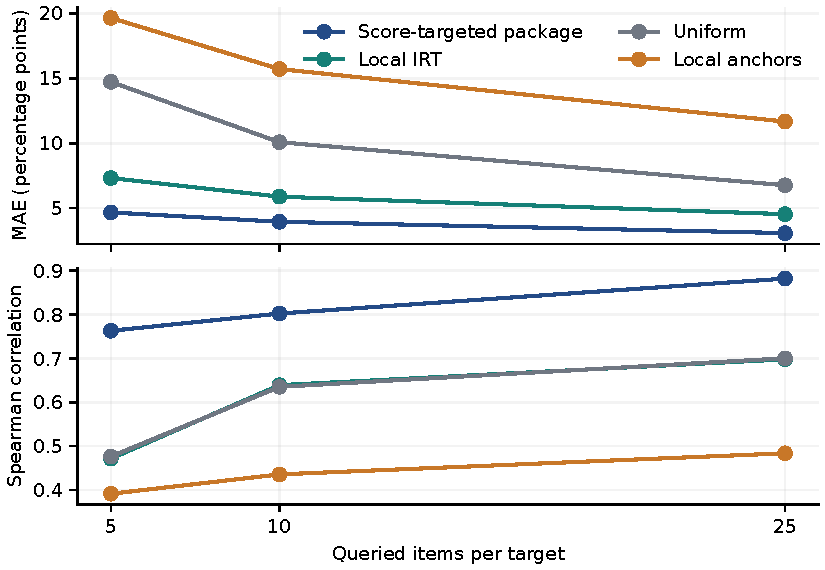
\includegraphics[width=\textwidth]{figures/budget_sensitivity.pdf}
\caption{Budget sensitivity, averaging over the same retained benchmarks and seeds. Top: absolute score error. Bottom: lineage-level Spearman correlation. Lines connect query budgets on nested paths, not an optimization history. The constant source prior is omitted from both panels to keep the common four-method legend readable.}
\label{fig:budget}
% @evidence[[analysis/paper_statistics.json#/by_budget]]
\end{figure}

\subsection{Paired Uncertainty, Seeds, and Controls}
For a given benchmark, errors are first averaged within each target lineage over its rows, query budgets, and seeds. The difference between package and comparator is formed before resampling. Lineage identifiers are sampled with replacement within each benchmark, and the sampled means are averaged with equal benchmark weights. The stored 200 draws give the 2.5th and 97.5th percentiles. Bootstrap randomness uses seed 1729. The four comparator intervals share this procedure, but are not presented as simultaneous confidence intervals. Repeating the same stored uncertainty object in seed records adds no information.
% @evidence[[source_evidence/evaluator/evaluate_final.py#L1065]]
% @evidence[[analysis/paper_statistics.json#/uncertainty]]

\begin{table}[ht]
\centering
\caption{Descriptive seed variation for the package, with equal benchmark and budget weights. Error units are percentage points. These seeds do not change the frozen data partitions.}
\label{tab:seeds}
% BEGIN GENERATED seeds
% @evidence[[analysis/paper_statistics.json#/by_seed]]
\begin{tabular}{rrrrr}
\toprule
Seed & MAE & RMSE & Spearman & Kendall\\
\midrule
1009 & 3.816 & 4.674 & 0.8238 & 0.6777 \\
2003 & 4.006 & 4.941 & 0.8148 & 0.6689 \\
3001 & 3.876 & 4.899 & 0.8089 & 0.6682 \\
\bottomrule
\end{tabular}
% END GENERATED seeds
% @evidence[[analysis/paper_statistics.json#/by_seed]]
\end{table}

The source prior produces identical predictions across target rows. A meaningful rank correlation is therefore undefined. The evaluator uses a negative sentinel for exact degeneracy, but floating-point differences in averages of identical values can also defeat that exact-equality test. We omit the prior's ranking outputs rather than interpreting such implementation artifacts as negative predictive association. The package and nonconstant comparator correlations in Table~\ref{tab:main} are reconstructed using the recorded lineage-mean convention.
% @evidence[[source_evidence/evaluator/evaluate_final.py#L562]]
% @evidence[[paper_data.json#/final_evaluation/evaluation_evidence/episodes]]

In the all-zero condition, queried values are overwritten without changing full-score references. In the rotated-source condition, each source row receives an independently drawn nonzero cyclic item shift, preserving row scores but breaking aligned item-response structure. A duplicate target with the same queried history checks row-position invariance; the normal BBH replay checks repeatability. Passing these checks constrains observed behavior, not all possible leakage or validity threats.
% @evidence[[source_evidence/evaluator/evaluate_final.py#L844]]
% @evidence[[source_evidence/evaluator/evaluate_final.py#L1040]]

\subsection{Reproduction and Evidence Boundaries}
The retained matrices originate from the supplied benchmark-prediction data snapshot at commit \texttt{55faff496947789f94e6b5908c77cbc3e84f81ad}. The frozen manifests preserve retained column indices, model rows, content normalization, lineage policy, and resource hashes. Raw upstream matrices alone do not reproduce the frozen splits without this metadata. The attached reproduction guide separates deterministic reconstruction of manuscript artifacts from an optional fresh evaluation, which was not run for this paper. It also documents the input resources required by the original evaluator rather than suggesting they can be recovered from scalar metrics.
% @evidence[[source_evidence/evaluator/rebuild.py]]
% @evidence[[source_evidence/manifests/bbh_manifest.json]]

Inspectability is provided by \path{source_evidence/selected/src/surrogate.py} (weighted statistics, acquisition, linear decoder, and tuning), \path{source_evidence/selected/src/nonlinear_decoder.py} (optional decoder and nested source fitting), and \path{source_evidence/selected/src/program.py} (observation interface). Locations are indexed in \path{source_evidence/LOCATIONS.md}; byte hashes and source-identity limitations are recorded in \path{source_evidence/inventory.json}. The evaluator definitions are in \path{source_evidence/evaluator/evaluate_final.py}. Hashes identify artifacts but are not substitutes for inspecting their content.

Numerical postprocessing uses NumPy \citep{Harris2020} and SciPy \citep{Virtanen2020}; plots use Matplotlib \citep{Hunter2007}. The analysis script reads the immutable evidence registry, excludes replay, reconciles aggregate metrics, and exports tables, vector PDF plots, PNG previews, and provenance sidecars. The conceptual figure is separately prepared from the manuscript's information-flow description, not from synthetic results. Literature consultation used direct permitted identifiers and abstracts, with no citation-network expansion. Inaccessible classical sources were not cited on metadata alone. No prohibited-study encounter was identified during this writing step; unsuccessful direct links are documented in the reproduction guide.

\subsection{LLM Usage}
LLM assistance was used to propose research designs, edit estimator implementations, plan reference queries, inspect supplied code and evaluator artifacts, synthesize the manuscript framing, write the LaTeX and plotting scripts, and check evidence links. The present manuscript step consulted directly retrieved literature abstracts and performed deterministic postprocessing of recorded predictions; it did not execute new model evaluations or component ablations. The conceptual overview is prepared through an automated diagram workflow. Evaluator-produced measurements are distinguished from LLM-generated interpretation and source descriptions. No independent human review or verification is claimed.

\end{document}
